\documentclass[10pt,twocolumn,letterpaper]{article}

\usepackage{statcourse}
\usepackage{times}
\usepackage{epsfig}
\usepackage{graphicx}
\usepackage{amsmath}
\usepackage{amssymb}


% Include other packages here, before hyperref.

% If you comment hyperref and then uncomment it, you should delete
% egpaper.aux before re-running latex.  (Or just hit 'q' on the first latex
% run, let it finish, and you should be clear).
\usepackage[breaklinks=true,bookmarks=false]{hyperref}


\statcoursefinalcopy


\setcounter{page}{1}
\begin{document}


%%%%%%%%%%%%%%%%%%%%%%%%%%%%%%%%%%%%%%%%%%%%%%%%%%%%%%%%%%%%%%%
% DO NOT EDIT ANYTHING ABOVE THIS LINE
% EXCEPT IF YOU LIKE TO USE ADDITIONAL PACKAGES
%%%%%%%%%%%%%%%%%%%%%%%%%%%%%%%%%%%%%%%%%%%%%%%%%%%%%%%%%%%%%%%



%%%%%%%%% TITLE
\title{Forecasting Stock Returns via Supervised Learning}

\author{Samuel Ilic\\
{\tt\small ilic@wisc.edu}
\and
Meenmo Kang\\
{\tt\small mkang84@wisc.edu}
\and
Jonathan Santoso\\
{\tt\small jsantoso2@wisc.edu@wisc.edu}
}

\maketitle
%\thispagestyle{empty}



% MAIN ARTICLE GOES BELOW
%%%%%%%%%%%%%%%%%%%%%%%%%%%%%%%%%%%%%%%%%%%%%%%%%%%%%%%%%%%%%%%


%%%%%%%%% ABSTRACT
\begin{abstract}
We apply several machine learning models to the prediction of stock prices, specifically the price of IBM stock. Decision trees such as Random Forest, Bagging, Boosting, and Linear Regression are conducted within our research as part of a comparative analysis in an attempt to arrive at the best model. Mean square error (MSE) is used as an indicator to evaluate the accuracy of the prediction. Through this process we arrived at the best models from each method whose $R^2$ is the highest and MSE is the lowest.

\end{abstract}

%%%%%%%%% BODY TEXT
\section{Introduction}

A primary reason why people are more passionate about analysis in financial fields than in other areas is that it is involves massive amounts of money. Various methodologies for predicting stock market activities have been developed over a long time, particularly via quantitative analysis by mathematicians in recent years. Moreover, as computing devices and computing ability have improved, machine learning has begun to be introduced in financial analysis. Compared to traditional statistical methods, machine learning has more flexibility to approximate random movements of data.

We therefore expected to arrive at enhanced predictions through several machine learning models, representing improvements over not only existing econometric approximation but also other market prediction methods.

The ultimate goal of our research is simply to find the best model to predict future stock returns. Decision trees have been selected for our research including Random Forest, Bagging, Boosting, and Linear Regression. These were highlighted in the class and we found these models to be a more viable and proper approach than other models for this case.

We specified a single stock; IBM was chosen for the project. IBM has a wealth of stock data history as it was long ago listed on NSYE and its price has been fluctuating, which implies there are many predictive factors, unlike the stock of consistently skyrocketing tech companies such as the FAANG (Facebook, Amazon, Apple, Netflix and Google) group. 


\subsection{Subsection}

You can use paragraphs or subsections to further structure your
main sections. This is an example of a subsection.

\paragraph{This is a paragraph title.} This is an example of a paragraph.

\section{Related Work}

Related work should be discussed here. This is an example of a citation \cite{mirjalili2018gender}. To format the citations properly, put the
corresponding references into the bibliography.bib file. You can obtain
BibTeX-formatted references for the "bib" file from Google Scholar 
(\url{https://scholar.google.com}), for example, by clicking on the 
double-quote character under a citation and then selecting \mbox{"BibTeX"} as
shown in Figure \ref{fig:google-scholar-1col} and 
Figure \ref{fig:google-scholar-2col}.

\begin{figure}[t]
\begin{center}
   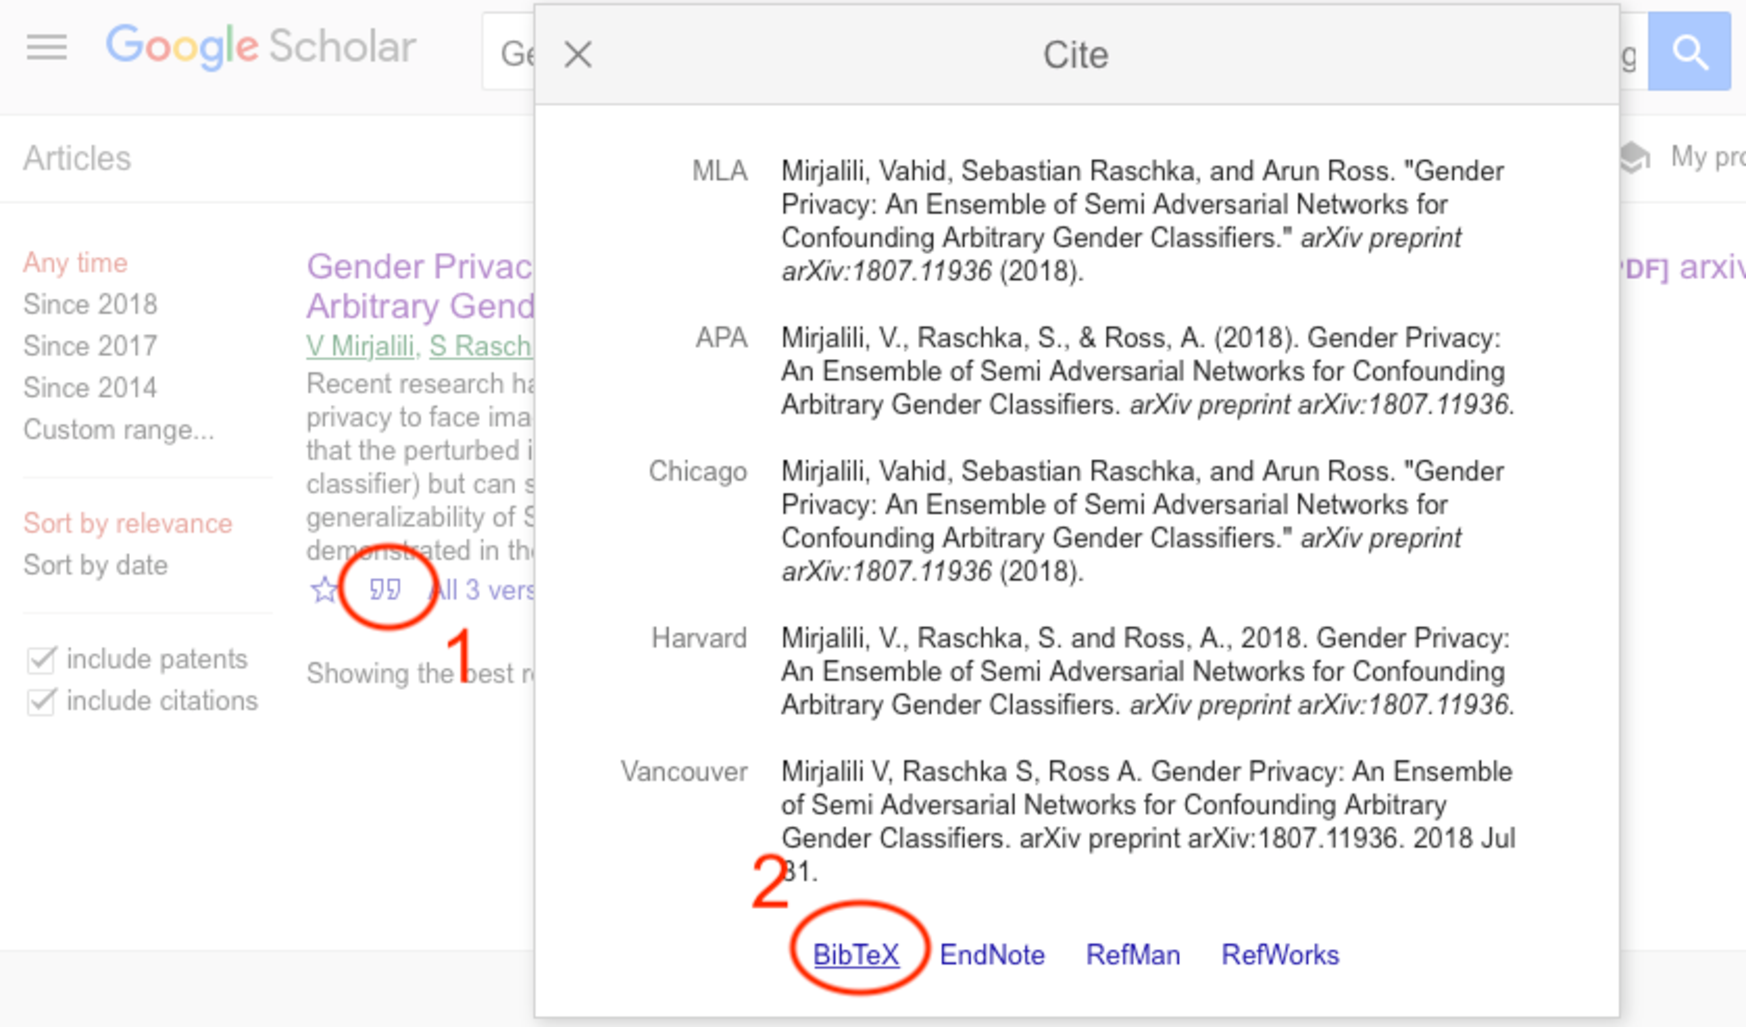
\includegraphics[width=0.8\linewidth]{Figures/google-scholar.pdf}
\end{center}
   \caption{Example illustrating how to get BibTeX references from
   Google Scholar as a 1-column figure.}
\label{fig:google-scholar-1col}
\end{figure}


\begin{figure*}
\begin{center}
   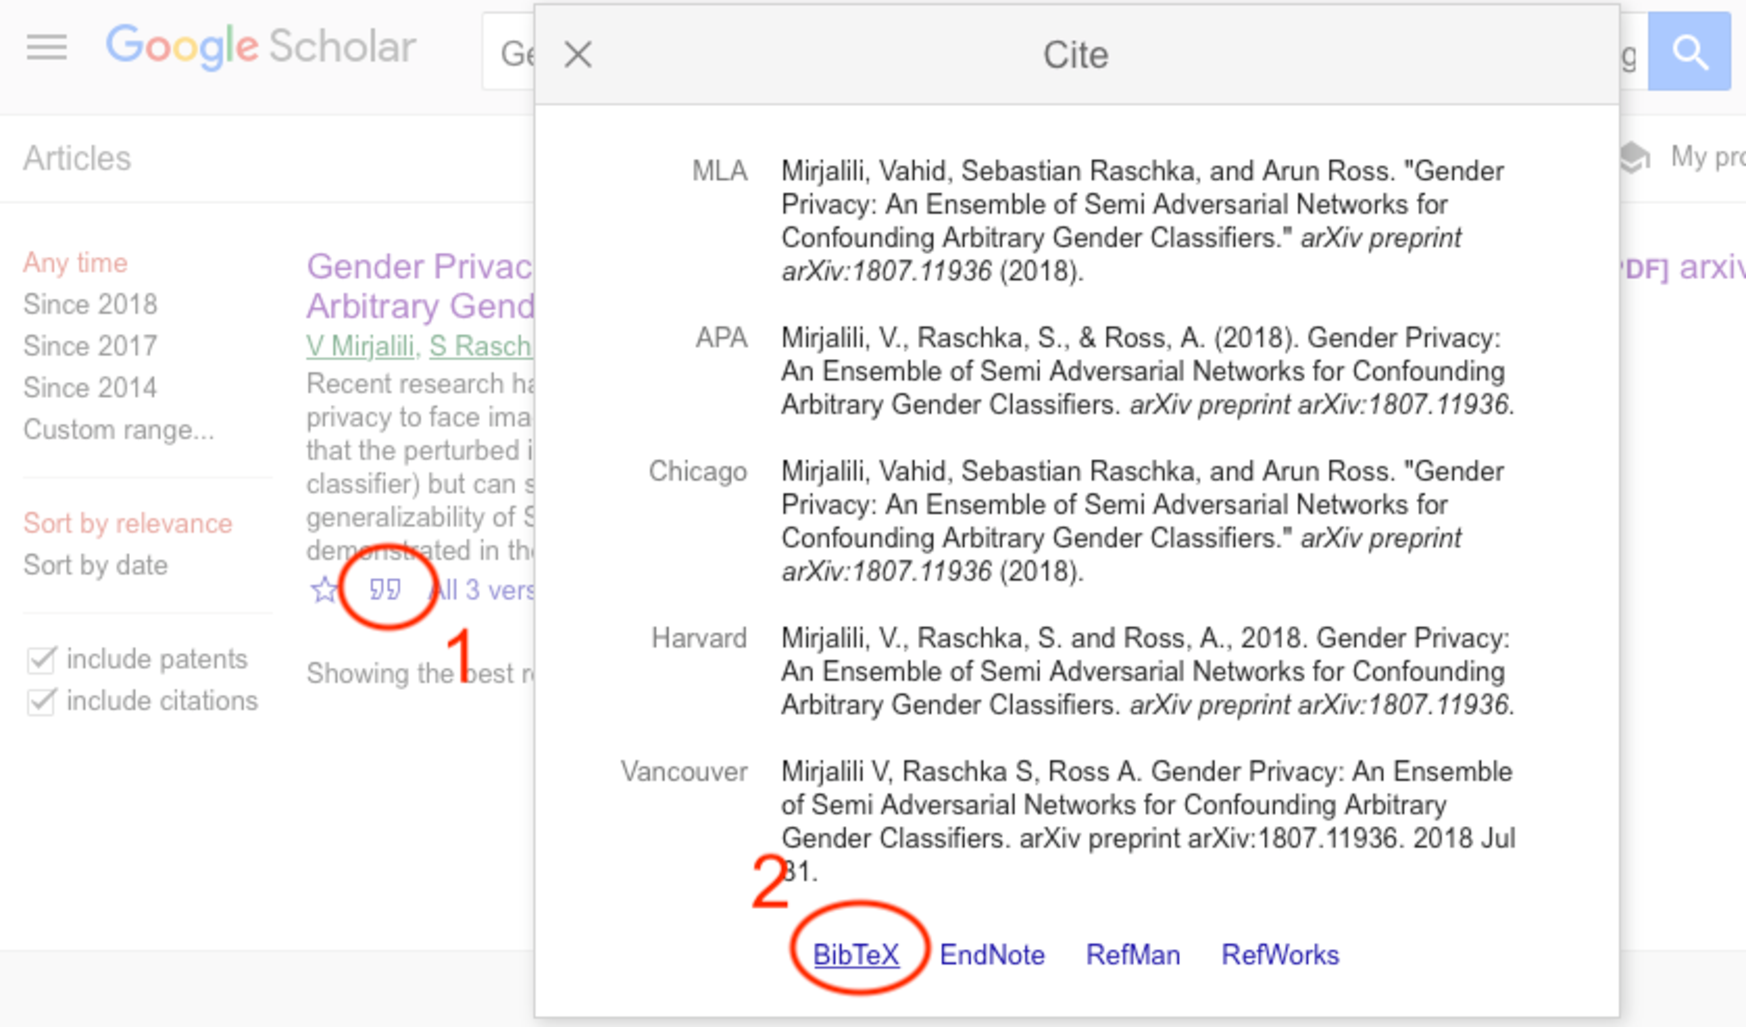
\includegraphics[width=0.8\linewidth]{Figures/google-scholar.pdf}
\end{center}
   \caption{Example illustrating how to get BibTeX references from
   Google Scholar as a 2-column figure.}
\label{fig:google-scholar-2col}
\end{figure*}

Table \ref{tab:some-table} shows an example for formatting a table.

\begin{table}
\begin{center}
\begin{tabular}{|l|c|}
\hline
Method & Accuracy \\
\hline\hline
Method 1 & $70 \pm 3$ \% \\
 Method 2 & $76 \pm 3$ \% \\
\hline
\end{tabular}
\end{center}
\label{tab:some-table}
\caption{This is an example of a table.}
\end{table}


\section{Proposed Method}

Describe the method(s) you are proposing, developing, or using. I.e., details
of the algorithms may be included here. 

\section{Experiments}

Describe the experiments you performed. You may want to create separate
subsections to further structure this section.

\subsection{Dataset}

Briefly describe your dataset in a separate subsection.


\subsection{Software}

Briefly list (and cite) software software you used.

\subsection{Hardware}

If relevant, list hardware resources you used.


\section{Results and Discussion}

Describe the results you obtained from the experiments and interpret them.
Optionally, you could split "Results and Discussion" into two separate
sections.

\section{Conclusions}

Describe your conclusions here. If there are any future directions, you can
describe them here, or you can create a new section for future directions.

\section{Acknowledgements}

List acknowledgements if any. For example, if someone provided you a dataset, or
you used someone else's resources, this is a good place to acknowledge
the help or support you received.

\section{Contributions}

Describe the contributions of each team member who worked on this project.


{\small
\bibliographystyle{ieee}
\bibliography{bibliography.bib}
}

\end{document}
